\newcommand{\ClassPath}{../VIU_TFM_LaTeX_template}
\documentclass{\ClassPath/viu-tfm-template}
\usepackage{multicol}

\definecolor{maincolor}{HTML}{f25416}

%--------------------------------------------------------------------------
% Definiciones necesarias Modifica con tus datos
%--------------------------------------------------------------------------
\def\nombre{Gómez Olivencia, Rubén}
\def\dni{78910013-A}
\def\titulo{Product backlog y Sprint backlog}
\def\titulacion{Máster Universitario en Desarrollo de Aplicaciones y Servicios Web}
\def\curso{2022-2023}

%Los siguientes son opcionales: si no se ponen, la portada cambia un poco. Ideal para escribir artículos/trabajos cortos
\def\dirige{}
\def\convocatoria{}
\def\asignatura{Gestión de proyectos en entornos ágiles}


% importar fichero de Bibliografía
%\addbibresource{Actividad_1.bib}

\begin{document}
    \graphicspath{{../VIU_TFM_LaTeX_template/}}

    \coverpage

    \tableofcontents

\chapter{Introducción}

Hoy en día es conveniente hacer uso de las \textbf{metodologías ágiles} cuando realizamos la gestión de un proyecto, ya que cuentan con una serie de ventajas que nos van a permitir dar una respuesta más rápida y flexible ante posibles cambios durante la vida de desarrollo del producto.

Las metodologías ágiles cuentan con una serie de ventajas entre las que podemos destacar:

\begin{itemize}
    \item Podremos entregar resultados funcionales al cliente cada poco tiempo y así obtener \textit{feedback} de lo realizado.
    \item Seremos capaces de dar una respuesta ágil y flexible ante posibles cambios que puedan surgir (cambios en los requisitos, ante bajas de personal asignado al proyecto, dificultades durante el desarrollo...).
    \item Tratar de evitar burocracia innecesaria, para centrarnos de esta manera en el producto y sus funcionalidades.
    \item Se trata de involucrar al cliente y colaborar con él para de esta manera conseguir un mayor valor al producto.
\end{itemize}

Con todo ello, se va a realizar la gestión de un proyecto que dará como resultado un gestor de contraseñas y documentación sensible basado en una plataforma web creada con \href{https://angular.io/}{Angular} y que hará uso como \textit{backend} del sistema \href{https://www.vaultproject.io/}{Vault} de la empresa \href{https://www.hashicorp.com/}{Hashicorp}.


\chapter{Historias de usuario}

Para comenzar con la gestión del proyecto debemos obtener los requisitos del cliente y transformarlos en las conocidas como “\textbf{historias de usuario}”.

En ellas plasmaremos, en un lenguaje que pueda entender el cliente, las funcionalidades que el producto debe tener, a las que asociaremos otros datos como son:

\begin{itemize}
    \item \textbf{Identificador único} para poder diferenciarlas del resto.
    \item Una \textbf{estimación de tiempos}
    \item \textbf{Prioridad} inicial para poder ordenarlas entre ellas.
    \item Se asignará a un desarrollador.
    \item Se añadirán posibles dependencias de otras historias de usuario.
    \item Una \textbf{descripción} de lo que se quiere conseguir.
    \item Unos \textbf{criterios de validación} por parte del cliente.
\end{itemize}

\section{Resultado del análisis realizado}

A continuación se van a plasmar las distintas “historias de usuario” obtenidas:

\begin{requisitostbl}{X[-1]X[-1]X[-1]X[1]X[-1]}
    ID & Estimación & Prioridad  & Asignación &  Dependencias \\
    1  & 15 horas & 1  & Ariane Olivencia &   \\

    Desarrollar “esqueleto” del interfaz web \\

    \textbf{Descripción}:
    Como usuario necesito un interfaz web para poder acceder a la aplicación y hacer uso de ella. Es la base del proyecto. \\

    \textbf{Criterios de validación}:
    El interfaz es \textit{responsive}, visualmente atractivo y funcional. \\
\end{requisitostbl}

\begin{requisitostbl}{X[-1]X[-1]X[-1]X[1]X[-1]}
    ID & Estimación & Prioridad  & Asignación &  Dependencias \\
    2  & 5 horas & 1  & Rubén Gómez & 1  \\

    Crear “login” de usuario \\

    \textbf{Descripción}:
    Como usuario quiero poder acceder a la aplicación utilizando como sistema de autenticación un usuario y contraseña.  \\

    \textbf{Criterios de validación}:
    Los valores introducidos serán autenticados contra el \textit{backend} que el cliente decida (base de datos o LDAP/Active Directory). \\
\end{requisitostbl}


\begin{requisitostbl}{X[-1]X[-1]X[-1]X[1]X[-1]}
    ID & Estimación & Prioridad  & Asignación &  Dependencias \\
    3  & 30 horas & 1  & Rafael Gómez & 2  \\

    Listado de secretos \\

    \textbf{Descripción}:
    Como usuario quiero poder obtener un listado de los secretos existentes para poder navegar por ellos y seleccionar el que me interese. \\

    \textbf{Criterios de validación}:
    \begin{itemize}
        \item El listado completo se obtiene mediante un árbol jerarquizado.
        \item Se puede navegar por el árbol seleccionando “directorios” que desplegarán a su vez su contenido.
        \item También se puede hacer como si fuera un explorador de archivos.
        \item Se puede buscar por el nombre de los secretos.
    \end{itemize}
    \\
\end{requisitostbl}

\vspace{20pt}

\begin{requisitostbl}{X[-1]X[-1]X[-1]X[1]X[-1]}
    ID & Estimación & Prioridad  & Asignación &  Dependencias \\
    4  & 10 horas & 2  & Carmen Olivencia & 2  \\

    Visualizar un secreto \\

    \textbf{Descripción}:
    Como usuario quiero acceder a un secreto para visualizar su contenido.  \\

    \textbf{Criterios de validación}:
    \begin{itemize}
        \item La visualización mostrará el secreto en formato HTML.
        \item Si un usuario accede a un secreto “bloqueado” lo debe saber y no se le permitirá editarlo.
        \item Al visualizar el secreto aparecerán botones con distintas acciones que se podrán realizar sobre él (editar, imprimir, ver históricos, borrar).
    \end{itemize}
    \\
\end{requisitostbl}


\begin{requisitostbl}{X[-1]X[-1]X[-1]X[1]X[-1]}
    ID & Estimación & Prioridad  & Asignación &  Dependencias \\
    5  & 25 horas & 2  & Rubén Gómez & 2  \\

    Modificar un secreto \\

    \textbf{Descripción}:
    Como usuario quiero poder editar un secreto para realizar modificaciones.  \\

    \textbf{Criterios de validación}:
    \begin{itemize}
        \item La modificación se realizará a través de un editor \textit{\textbf{WYSIWYG}}.
        \item El editor permitirá realizar modificaciones en formato \href{https://es.wikipedia.org/wiki/Markdown}{Markdown}.
        \item El editor permitirá guardar el secreto y al hacerlo volveremos a la visualización del mismo.
        \item Al comenzar la modificación el secreto se pondrá en estado “bloqueado”.
    \end{itemize}
    \\
\end{requisitostbl}

\vspace{10pt}

\begin{requisitostbl}{X[-1]X[-1]X[-1]X[1]X[-1]}
    ID & Estimación & Prioridad  & Asignación &  Dependencias \\
    6  & 10 horas & 3  & Asier Gómez & 4  \\

    Borrado de secretos \\

    \textbf{Descripción}:
    Como usuario quiero poder borrar secretos para que desaparezcan.  \\

    \textbf{Criterios de validación}:
    Antes de borrar debe existir un mensaje de confirmación. \\
\end{requisitostbl}

\vspace{10pt}

\begin{requisitostbl}{X[-1]X[-1]X[-1]X[1]X[-1]}
    ID & Estimación & Prioridad  & Asignación &  Dependencias \\
    7  & 15 horas & 3  & Ariane Olivencia & 2  \\

    Permitir gestionar ficheros como secretos \\

    \textbf{Descripción}:
    Como usuario quiero poder subir ficheros al sistema para guardarlos cifrados.  \\

    \textbf{Criterios de validación}:
    Se permite subir cualquier tipo de fichero y se podrá descargar. Se debe poder visualizar los ficheros más habituales en la propia web (imágenes y ficheros PDF) sin necesidad de descargarlos. \\
\end{requisitostbl}





\begin{requisitostbl}{X[-1]X[-1]X[-1]X[1]X[-1]}
    ID & Estimación & Prioridad  & Asignación &  Dependencias \\
    8  & 20 horas & 4  & Rafael Gómez & 4  \\

    Versionado de secretos\\

    \textbf{Descripción}:
    Como usuario quiero poder ver las veces que el fichero ha sido modificado para poder ver los cambios realizados.  \\

    \textbf{Criterios de validación}:
    \begin{itemize}
        \item Poder ver el número de versiones que tiene un secreto.
        \item Poder ver una versión concreta del secreto.
        \item Poder ver las diferencias entre versiones.
        \item Poder restaurar una versión concreta del secreto.
    \end{itemize} \\
\end{requisitostbl}






\begin{requisitostbl}{X[-1]X[-1]X[-1]X[1]X[-1]}
    ID & Estimación & Prioridad  & Asignación &  Dependencias \\
    9  & 5 horas & 4  & Asier Gómez & 2  \\

    Imprimir secretos \\

    \textbf{Descripción}:
    Como usuario quiero poder imprimir un secreto. \\

    \textbf{Criterios de validación}:
    Existe un botón para imprimir un secreto. \\
\end{requisitostbl}



\begin{requisitostbl}{X[-1]X[-1]X[-1]X[1]X[-1]}
    ID & Estimación & Prioridad  & Asignación &  Dependencias \\
    10  & 35 horas & 2  & Rubén Gómez & 1  \\

    Puesta en producción segura \\

    \textbf{Descripción}:
    Como usuario quiero poder acceder a la plataforma de manera segura para realizar todo lo comentado hasta ahora \\

    \textbf{Criterios de validación}:
    \begin{itemize}
        \item El acceso web tiene que ser por HTTPS (certificado válido).
        \item El servidor debe estar securizado ante accesos externos.
        \item Los servicios deben auto-arrancarse en caso de caída.
        \item Existe un registro de lo sucedido a cada secreto (auditoría).
    \end{itemize} \\
\end{requisitostbl}


\section{Mapa de las historias de usuario}

Dado que las historias de usuario pueden suponer la agrupación de distintas tareas técnicas que son más pequeñas, es conveniente crear un mapa que englobe todas las tareas a realizar.

Para la organización de este mapa se pueden identificar los siguientes apartados:
\begin{itemize}
    \item \textbf{Backbone} o temas, que son las características a alto nivel que va a tener la aplicación. En el mapa se ha diferenciado en color verde.
    \item Los \textbf{epics}, en color azul, son características que normalmente no pueden realizarse en un \textit{sprint} y que también pueden ser divididas en distintas historias de usuarios que están relacionadas entre sí.
    \item Las \textbf{tareas}, en este caso en amarillo, son las unidades concretas de trabajo, tratando que sean lo más cortas posibles y que a nivel técnico sean auto-contenidas y aisladas.
\end{itemize}

El mapa resultante es el siguiente:

\begin{center}
    %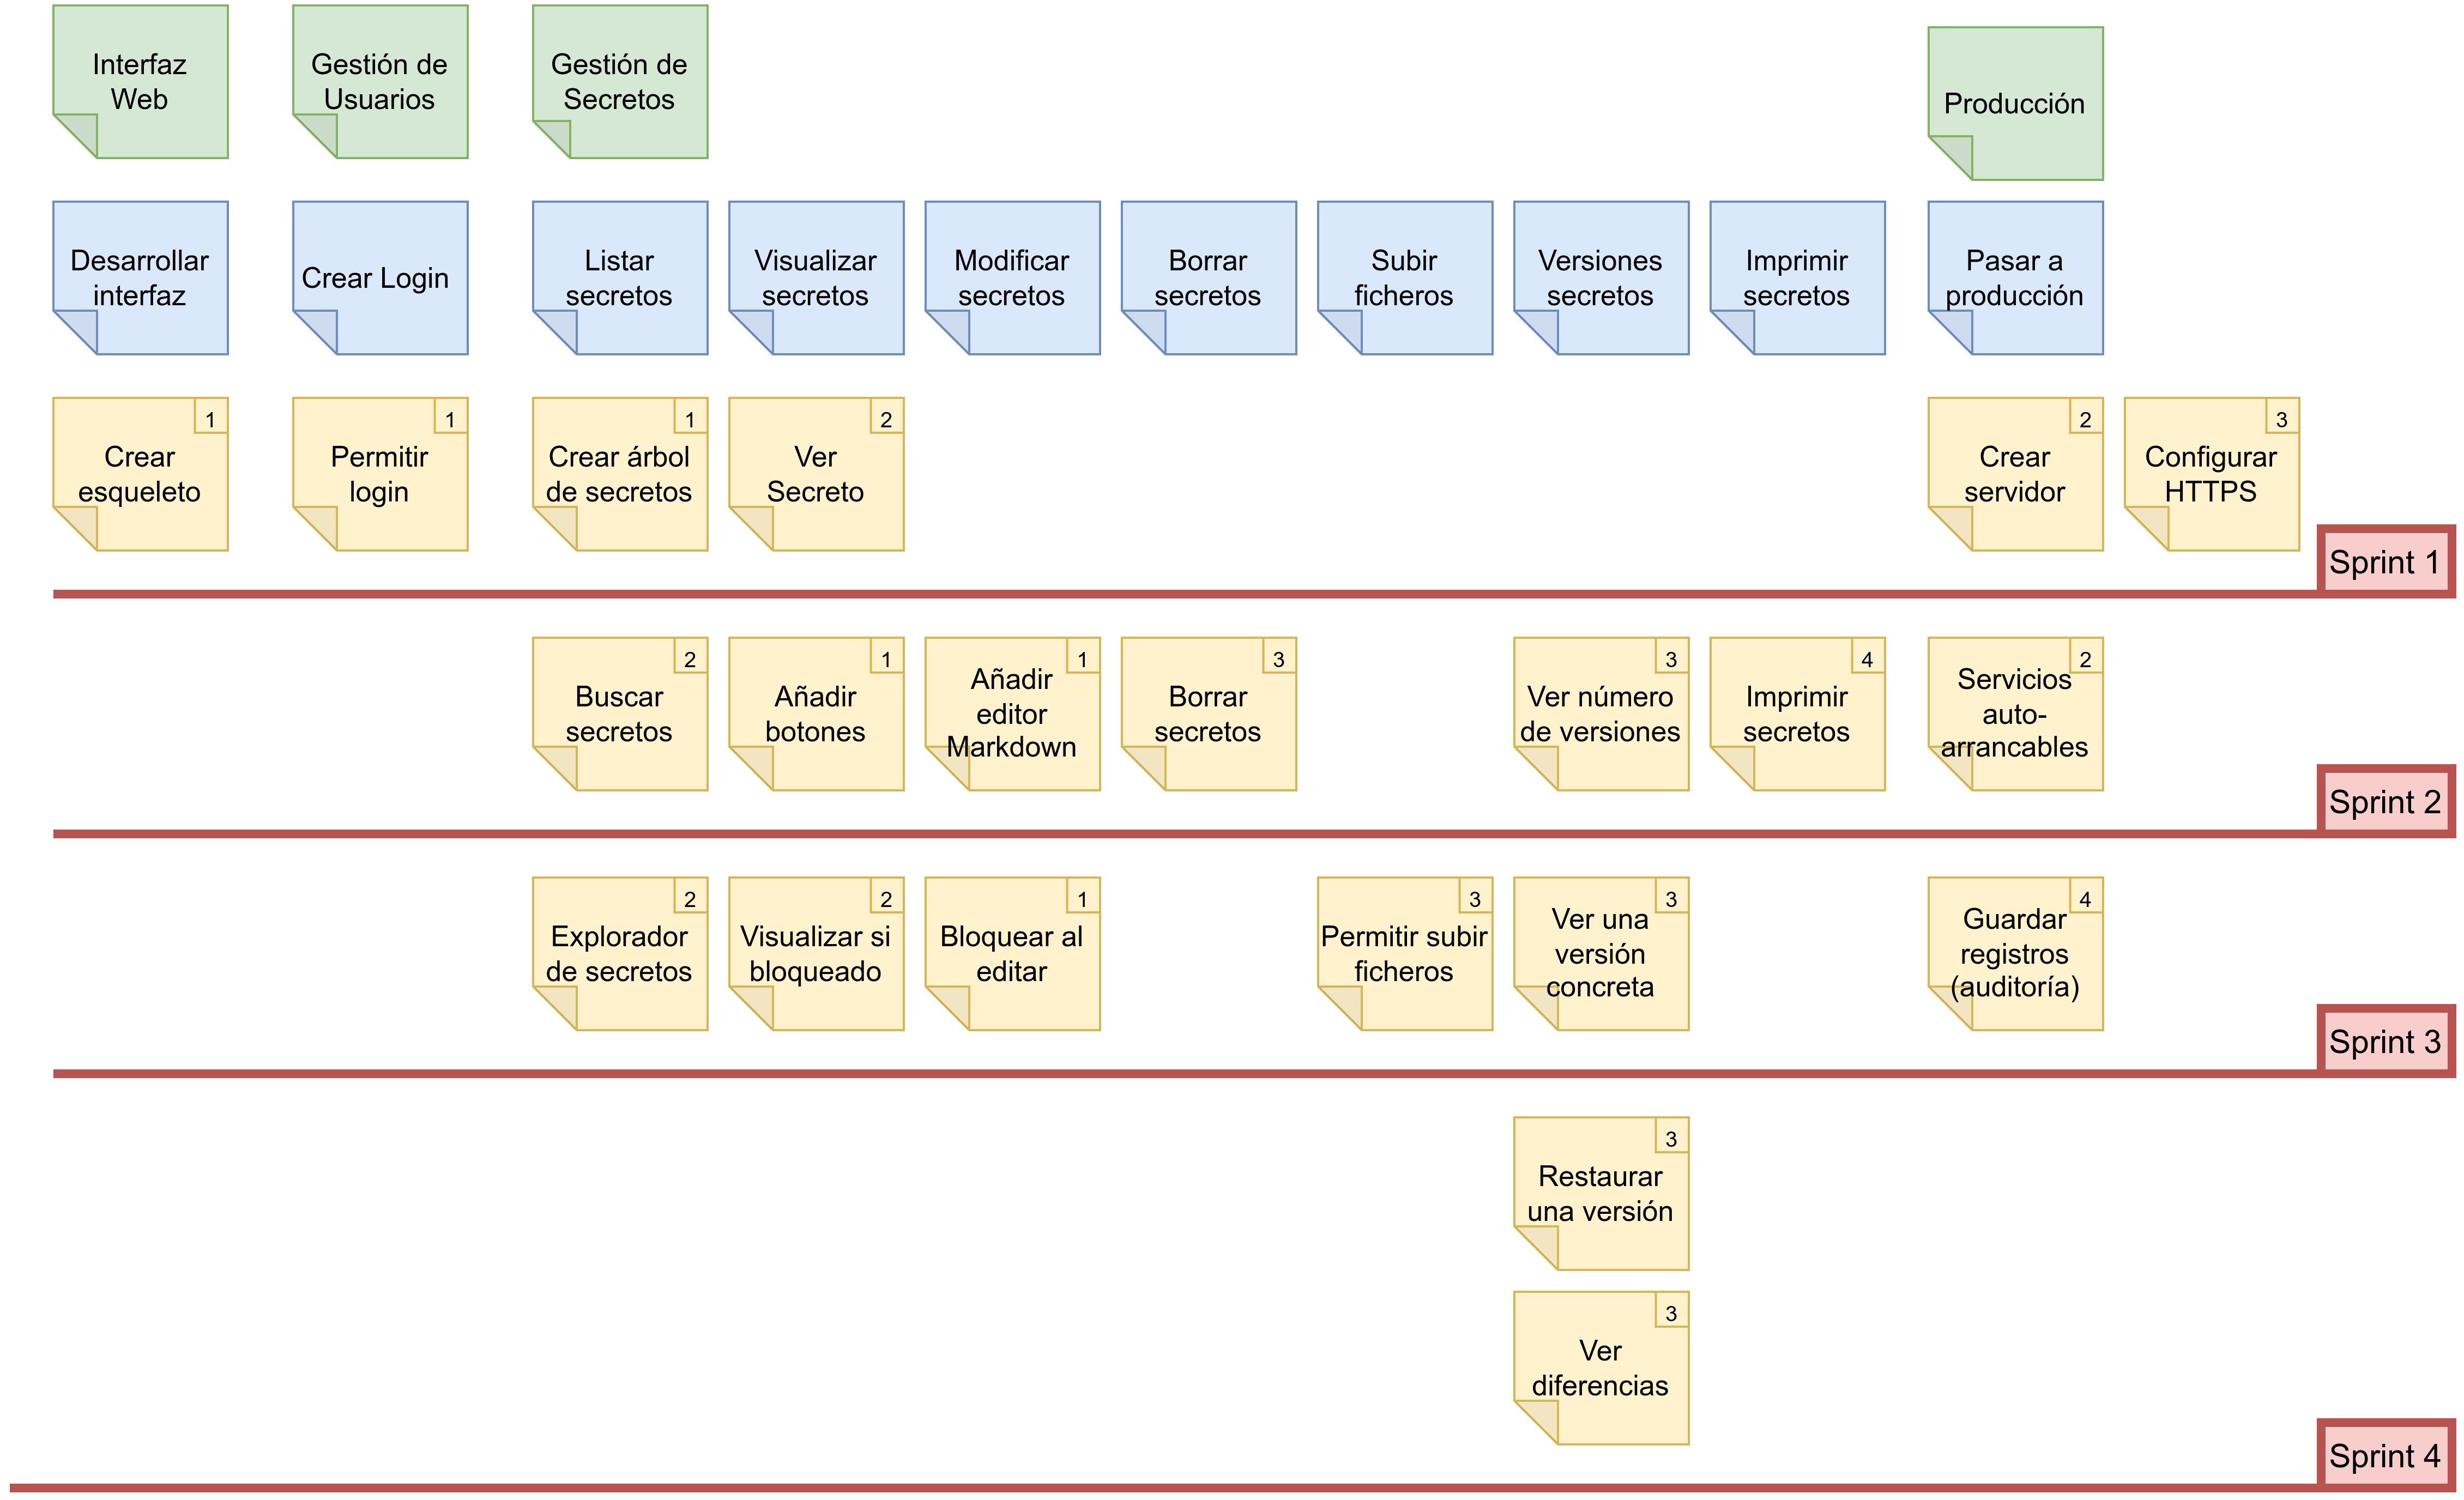
\includegraphics[angle=90,height=\textheight]{img/kanban.png}
    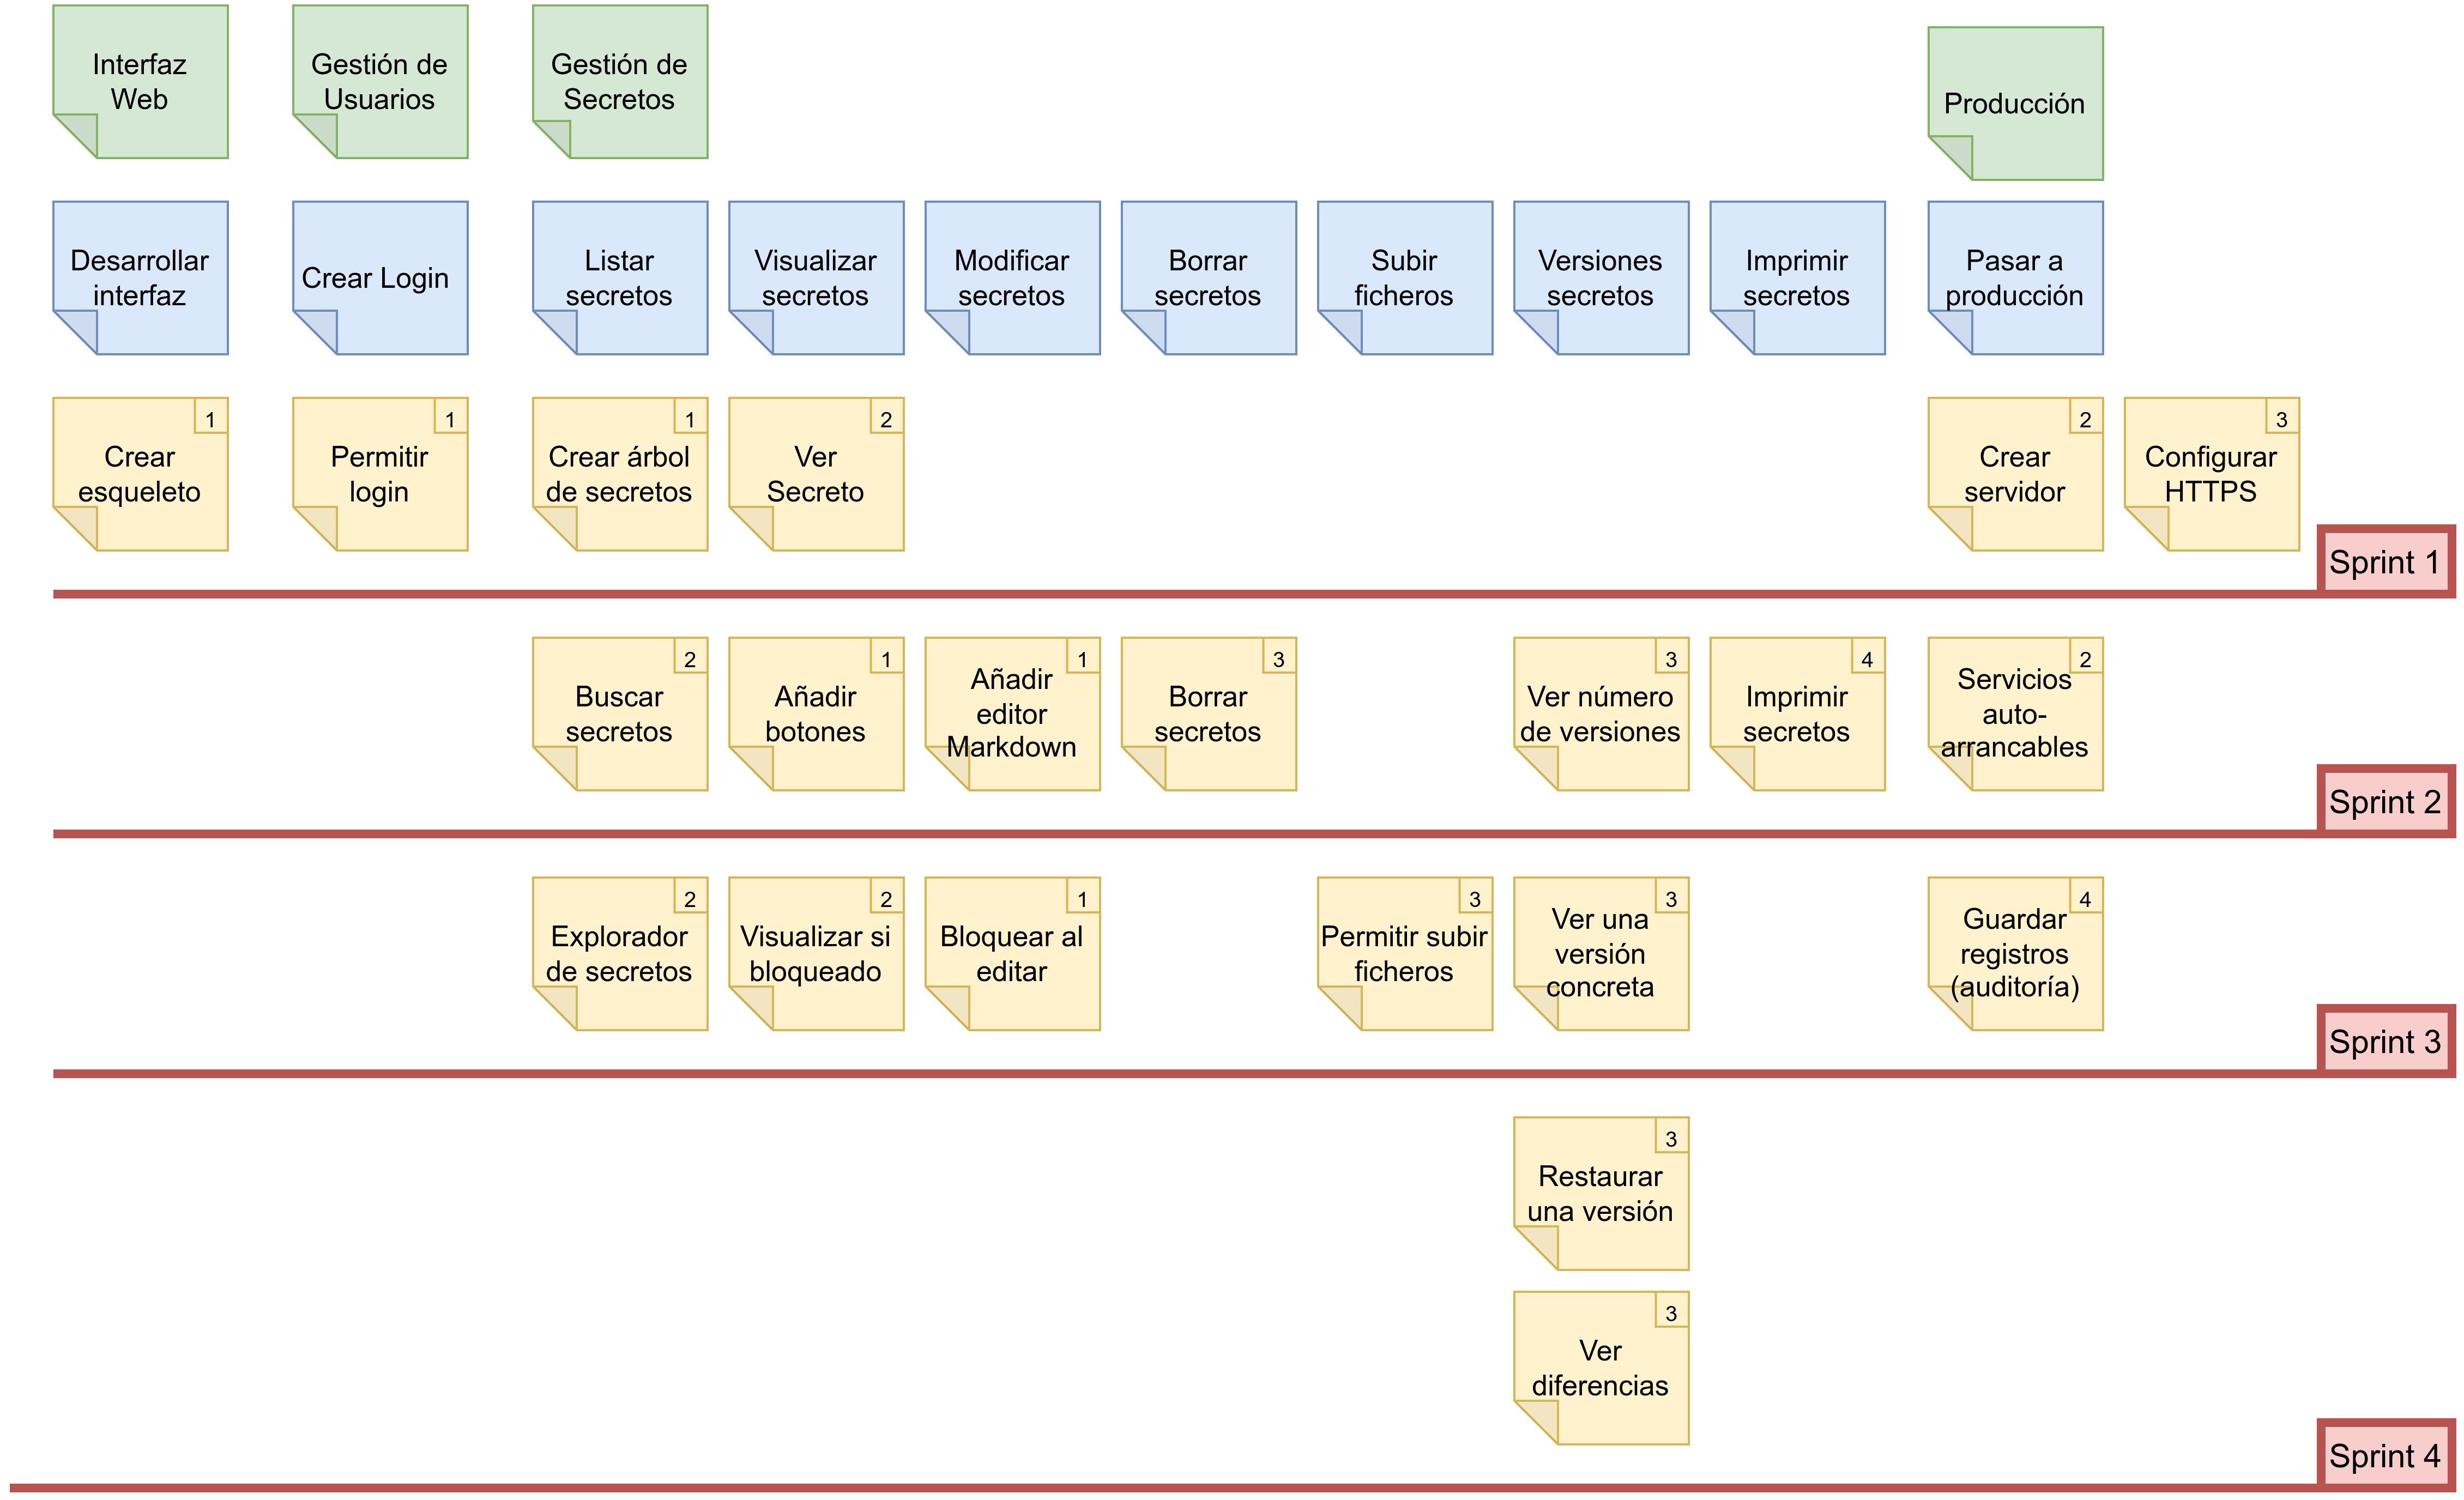
\includegraphics[width=\linewidth]{img/kanban.png}
\end{center}

\section{Sprint backlog}

A la par que se ha ido creando el mapa anterior, se han diferenciado diferentes \textit{sprints} con las tareas que deberían completarse para cada uno de ellos.

Bien es cierto, que aunque esa primera estimación haya sido realizada, se podrían efectuar modificaciones en caso de que fuese necesario.

Para el primer \textit{sprint} se han identificado las siguientes tareas que deben realizarse:

\begin{center}
    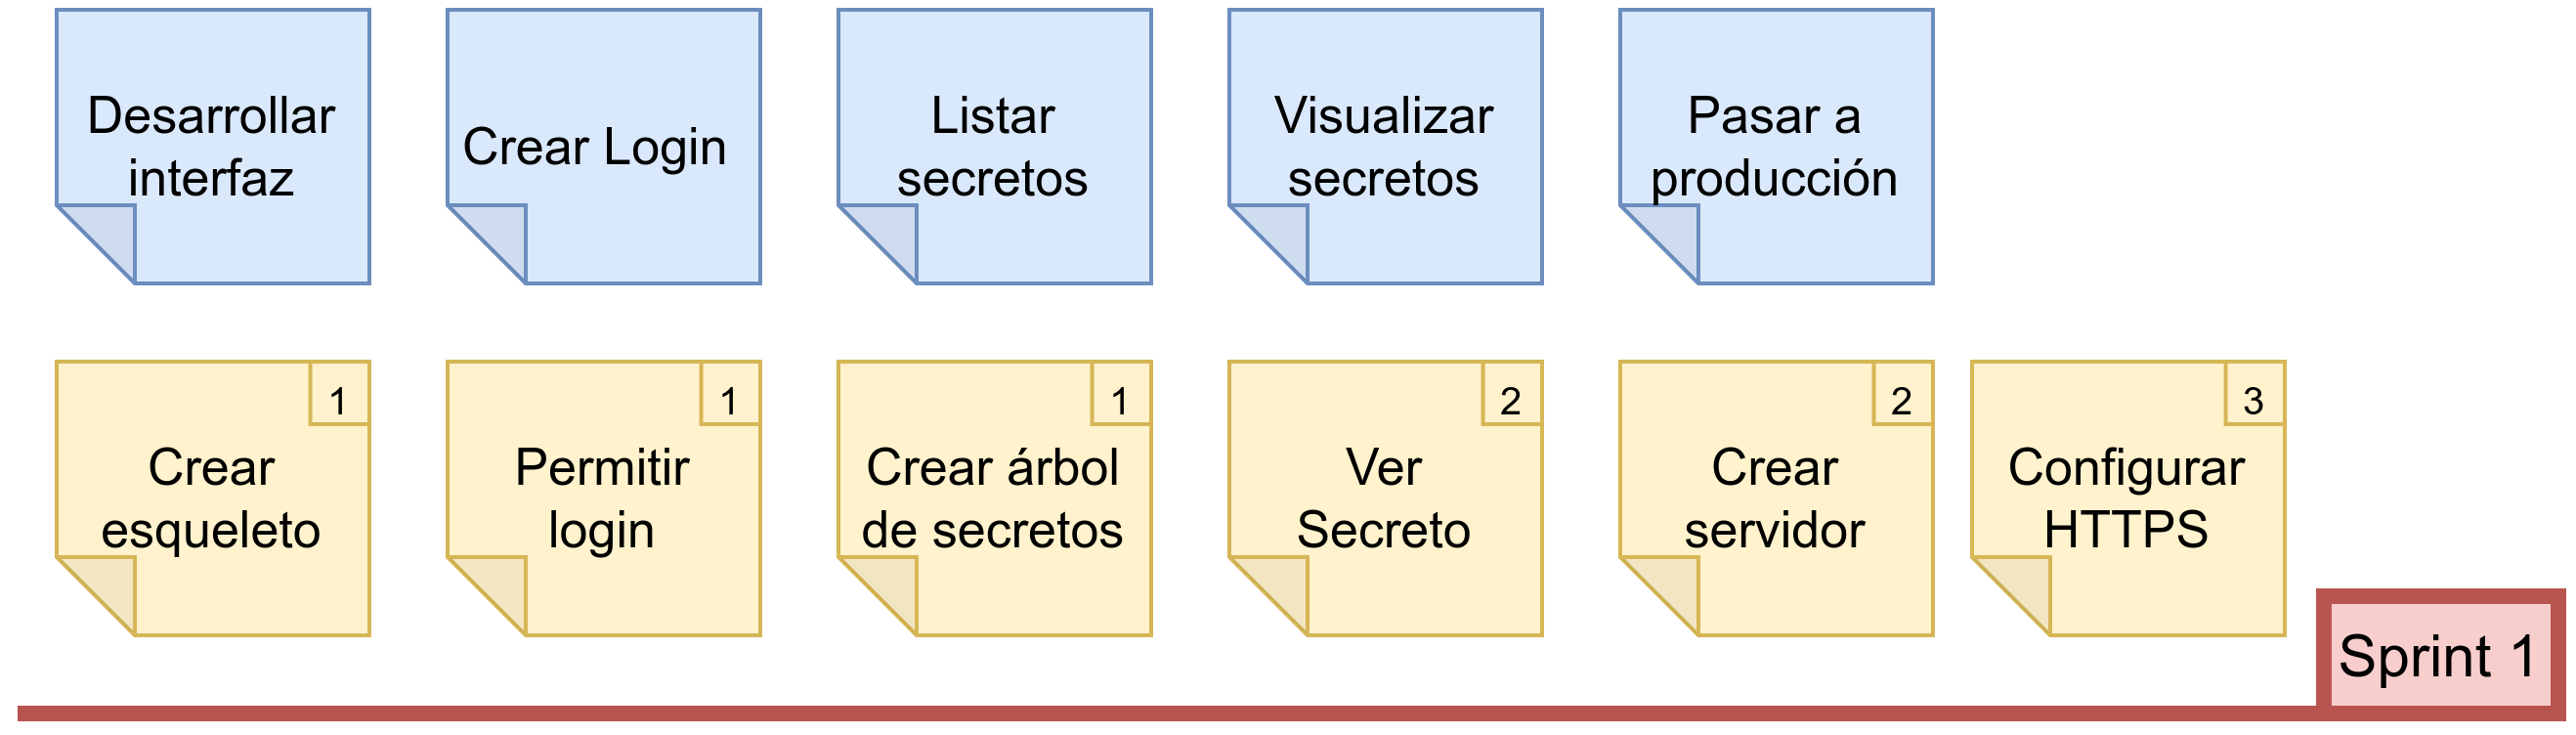
\includegraphics[width=\linewidth]{img/sprint1.png}
\end{center}

Tal como se puede ver, las tareas están representadas con su prioridad dentro del \textit{sprint}, para así también tener claro qué tareas deben tratar de terminarse antes que otras.

Al terminar este primer \textit{sprint}, tendremos la base del proyecto terminada, podremos mostrarle al cliente una primera versión con unas funcionalidades básicas.

De esta manera, el cliente nos puede dar \textit{feedback} de lo realizado, con una base ya terminada.Ese \textit{feedback} podremos utilizarlo como retroalimentación para el siguiente \textit{sprint}, ya sea para realizar modificaciones de lo ya realizado (hacer cambios nuevos que el cliente pida) o para utilizarlo para las tareas ya planificadas.


\chapter{Gestión de tareas en Trello}

\href{https://trello.com/}{Trello} es una aplicación web, creada por la empresa \href{https://www.atlassian.com/}{Atlassian}, que nos permite tener un tablero \href{https://en.wikipedia.org/wiki/Kanban_(development)}{Kanban} donde podremos añadir las tareas de nuestro proyecto, e ir moviéndolas entre distintas etapas.

Aunque cuenta con una versión de suscripción, la versión gratuita cuenta con las características suficientes como para poder ser utilizado para la gestión de proyectos sin problema alguno.

Una vez definidas las tareas, tal como se ha visto antes, se han añadido a Trello, en el que se han creado las siguientes columnas, o fases de desarrollo:

\begin{itemize}
    \item \textbf{Tareas pendientes}: donde situaremos las tareas que se deben realizar para llevar a cabo el proyecto.
    \item \textbf{Desarrollo}: Son las tareas que se han empezado a desarrollar.
\end{itemize}

\begin{minipage}{0.6\linewidth}
    \begin{itemize}

        \item \textbf{Testing}: Son las tareas que se dan por terminadas en el desarrollo y que pasan a una fase de testeo. En algunos casos puede ser directamente testeado por el cliente para dar su feedback (por ejemplo para el interfaz web), aunque lo habitual es que el testeo lo realice otra persona del proyecto (que no haya sido quien ha hecho el desarrollo).

        En caso de que una tarea no pase esta fase, se anotará los inconvenientes y volverá a la columna de \textbf{desarrollo}.
        \item \textbf{Producción}: Una vez el \textit{testing} ha terminado, se puede dar por terminada la tarea y debe ser incluida en producción.
    \end{itemize}
\end{minipage}
\hfill
\begin{minipage}{0.29\linewidth}
    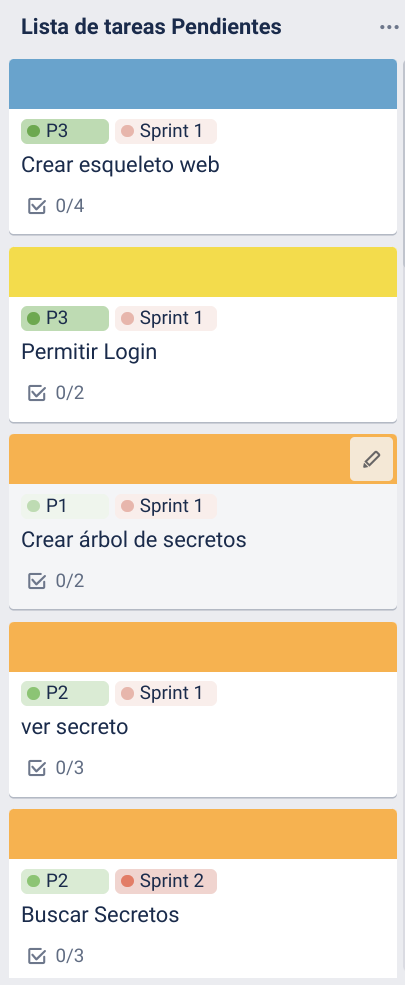
\includegraphics[width=\linewidth]{img/tareas.png}
    \vspace{-35pt}
    \begin{center}
        {\scriptsize \textit{Tareas pendientes en Trello}}
    \end{center}
\end{minipage}

\vspace{10pt}
Tal como se puede ver en la imagen, cada tarea se representa como una pequeña tarjeta, apareciendo como un listado de todas ellas en la columna correspondiente en las que están situadas (en este caso todavía en la tarea de pendientes).

A cada una de las tareas se les ha asignado un color y varias etiquetas que se van a detallar a continuación. De esta manera, Trello nos permitirá realizar búsquedas o visualizar las tareas con la etiqueta que nos interese.


\begin{minipage}{0.48\linewidth}
    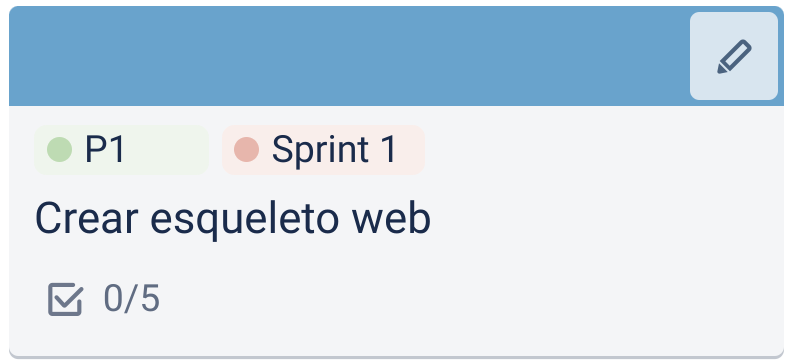
\includegraphics[width=\linewidth]{img/tarea.png}
    \vspace{-35pt}
    \begin{center}
        {\scriptsize \textit{Detalle de tarea}}
    \end{center}
\end{minipage}
\hfill
\begin{minipage}{0.47\linewidth}
    A cada tarjeta se le ha dado un color, dependiendo del tema al que esté más orientada la tarea.

    Otro aspecto son las etiquetas asignadas. En este caso cuenta con “\textbf{P1}” que marca la prioridad, siendo esta la más alta, y la segunda etiqueta referenciando a qué \textit{sprint} pertenece.
\end{minipage}

Por último, cada tarea puede tener pequeños ítems. Estos han sido detalladas para que el desarrollador tenga en cuenta qué es lo que debe hacer para dar por finalizada la tarea.

Tal como se ha dicho previamente se pueden hacer filtros por las etiquetas, por lo que dependiendo del \textit{sprint} en el que nos encontremos, podremos filtrar por dicha etiqueta, quedando el inicio del primer \textit{sprint} de la siguiente manera:

\begin{center}
    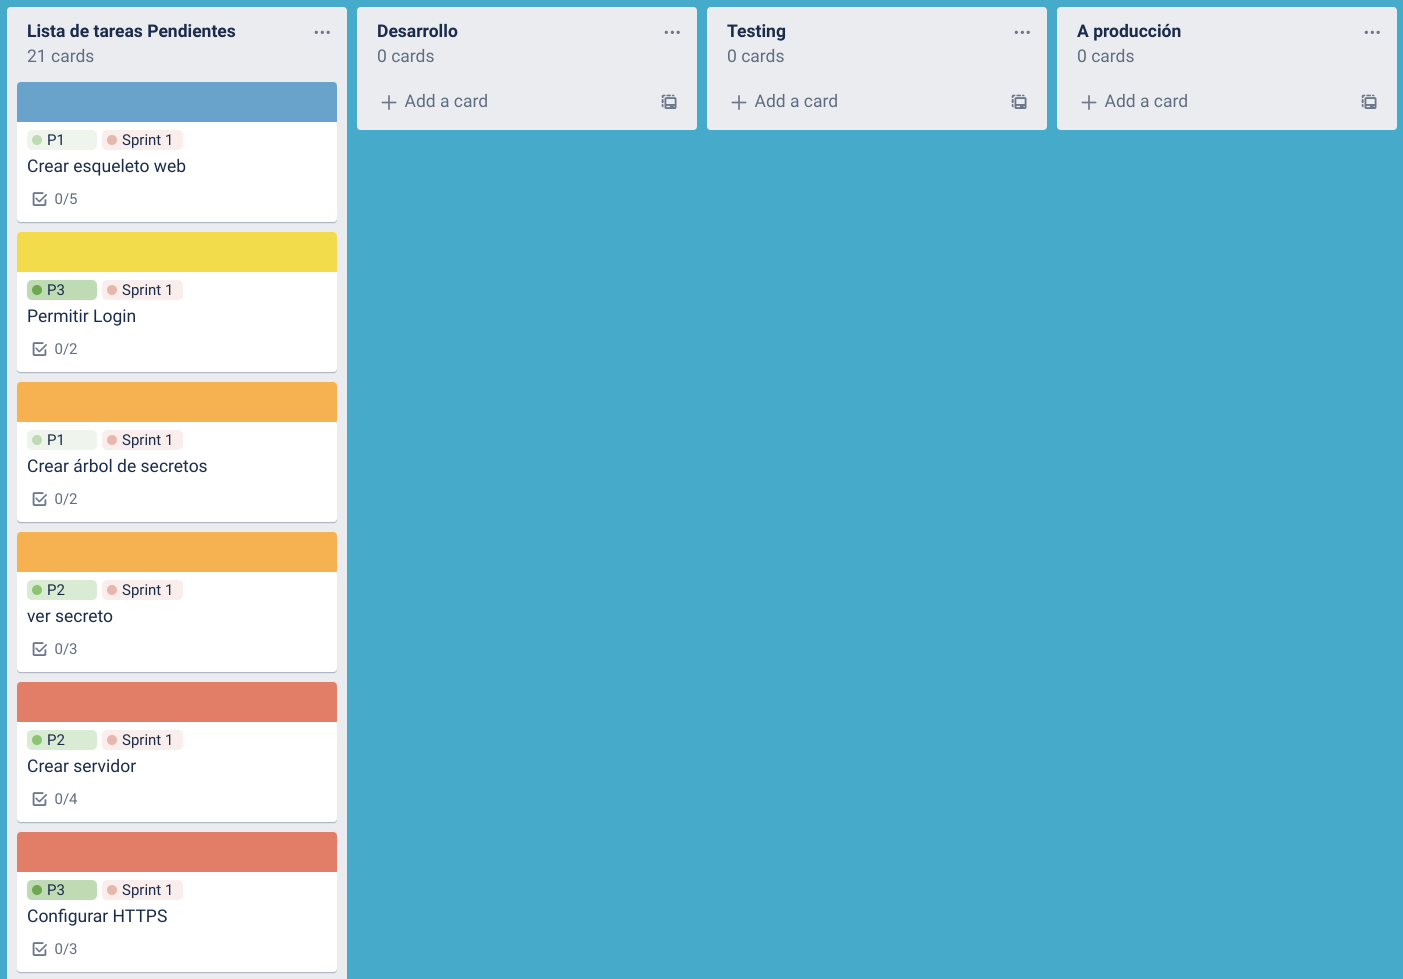
\includegraphics[frame,width=0.9\linewidth]{img/board1.png}
\end{center}

Este es el punto de partida y las tareas serán repartidas a sus correspondientes desarrolladores, que empezarán con ellas en cuanto se termine la asignación.

\section{Avance de tareas}
Tras asignar las primeras tareas, estas son movidas a la columna “desarrollo”.

\begin{center}
    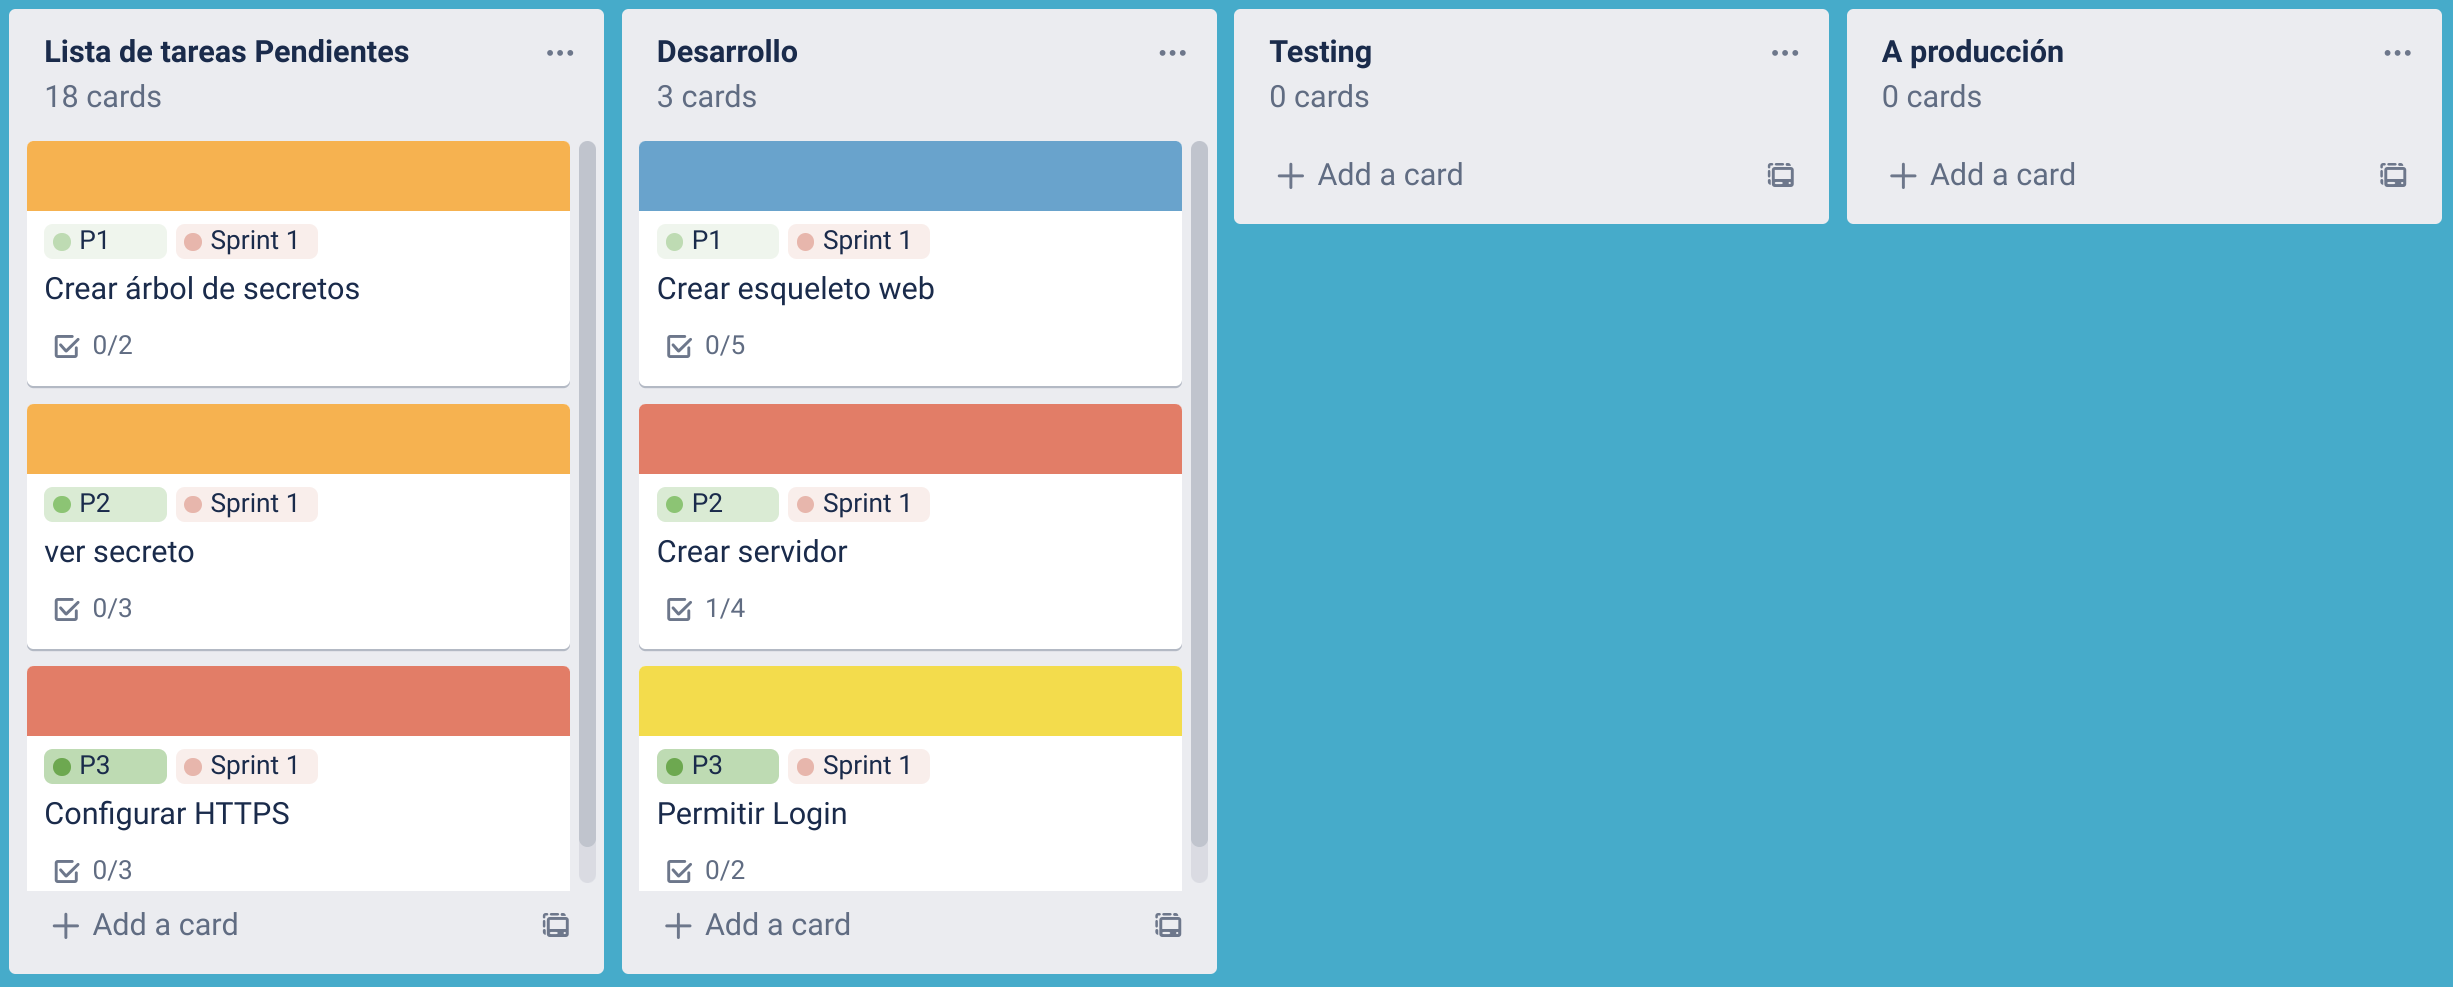
\includegraphics[width=0.9\linewidth]{img/board2.png}
\end{center}

De esta manera, los desarrolladores comenzarán a realizar los ítems que tiene sus tareas. A continuación se muestran los ítems de las primeras tres tareas:

{
    \begin{minipage}{0.32\linewidth}
        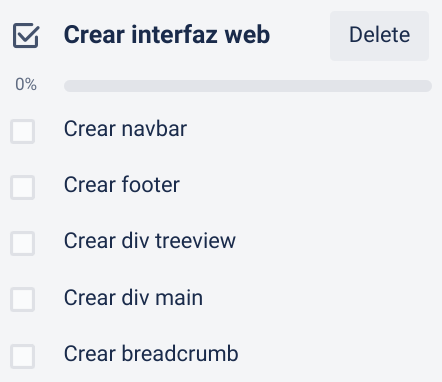
\includegraphics[width=\linewidth]{img/tarea1.png}
    \end{minipage}
    \hfill
    \begin{minipage}{0.32\linewidth}
        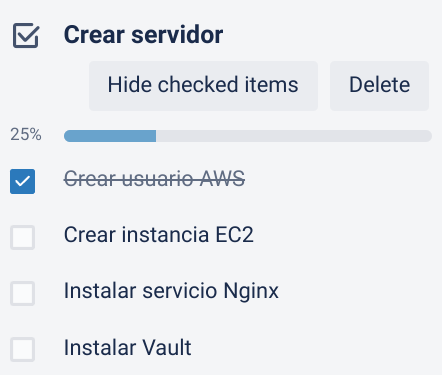
\includegraphics[width=\linewidth]{img/tarea2.png}
    \end{minipage}
    \hfill
    \begin{minipage}{0.32\linewidth}
        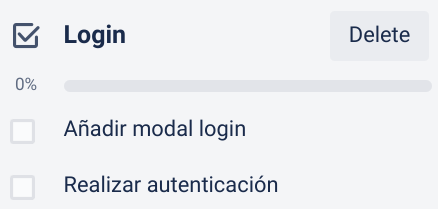
\includegraphics[width=\linewidth]{img/tarea3.png}
    \end{minipage}
}

Como se puede ver, en la tarea de “Crear servidor” ya ha habido un pequeño avance porque se ha creado el usuario en el servicio \href{https://aws.amazon.com/es/}{AWS} de Amazon.

Si dejamos avanzar un poco el tiempo, el panel avanzará a tener el siguiente aspecto:

\begin{center}
    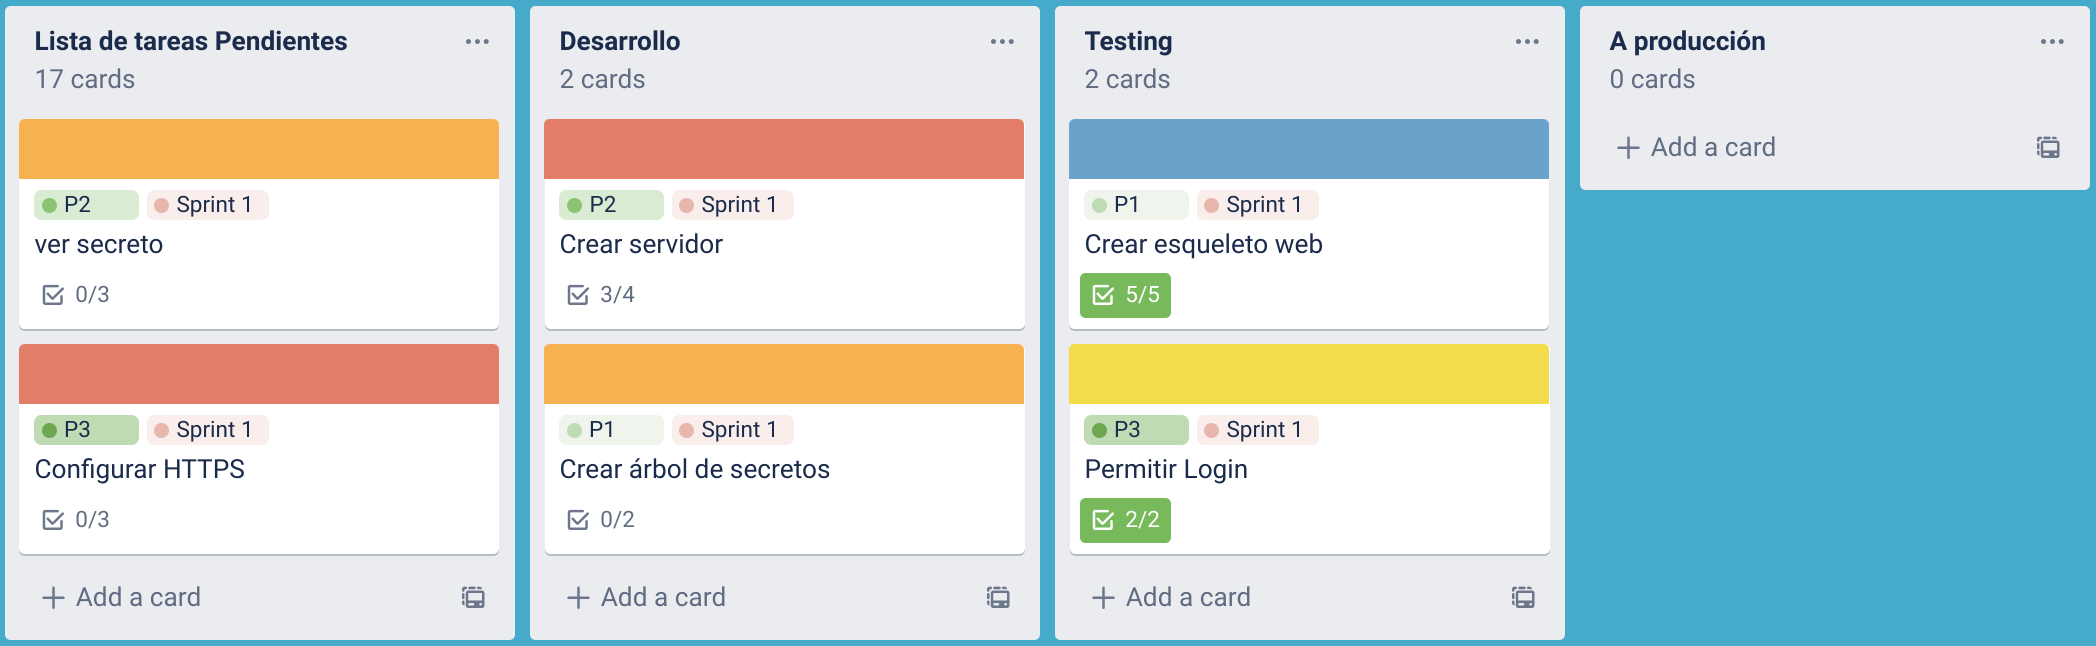
\includegraphics[width=\linewidth]{img/board3.png}
\end{center}

En este punto en el que nos encontramos, se puede ver cómo ha habido un avance de dos tareas a la columna “\textit{\textbf{Testing}}”. Esto significa que se han completado todos los ítems 
\includegraphics[height=1.3em]{img/items.png} en cada tarea :
\begin{itemize}
    \item \textbf{Crear esqueleto web} es la tarea inicial que crea la web para el desarrollo del proyecto. En este caso el testing va a ser llevado por parte del cliente para que ofrezca su \textit{feedback} de lo realizado y por si quiere realizar algún tipo de cambio en colores o maquetación.

    \item \textbf{Permitir login} es la otra tarea completada y que por tanto debe testearse. Esta tarea debe testearse de manera correcta ya que es importante de cara al resto del proyecto.
\end{itemize}

En desarrollo sigue la tarea “crear servidor”, aunque ahora mismo se encuentra al 75\% y se ha comenzado a desarrollar la tarea “crear árbol de secretos”.

Si dejamos avanzar un poco más el tiempo el panel llega a tener este aspecto:

\vspace{-10pt}
\begin{center}
    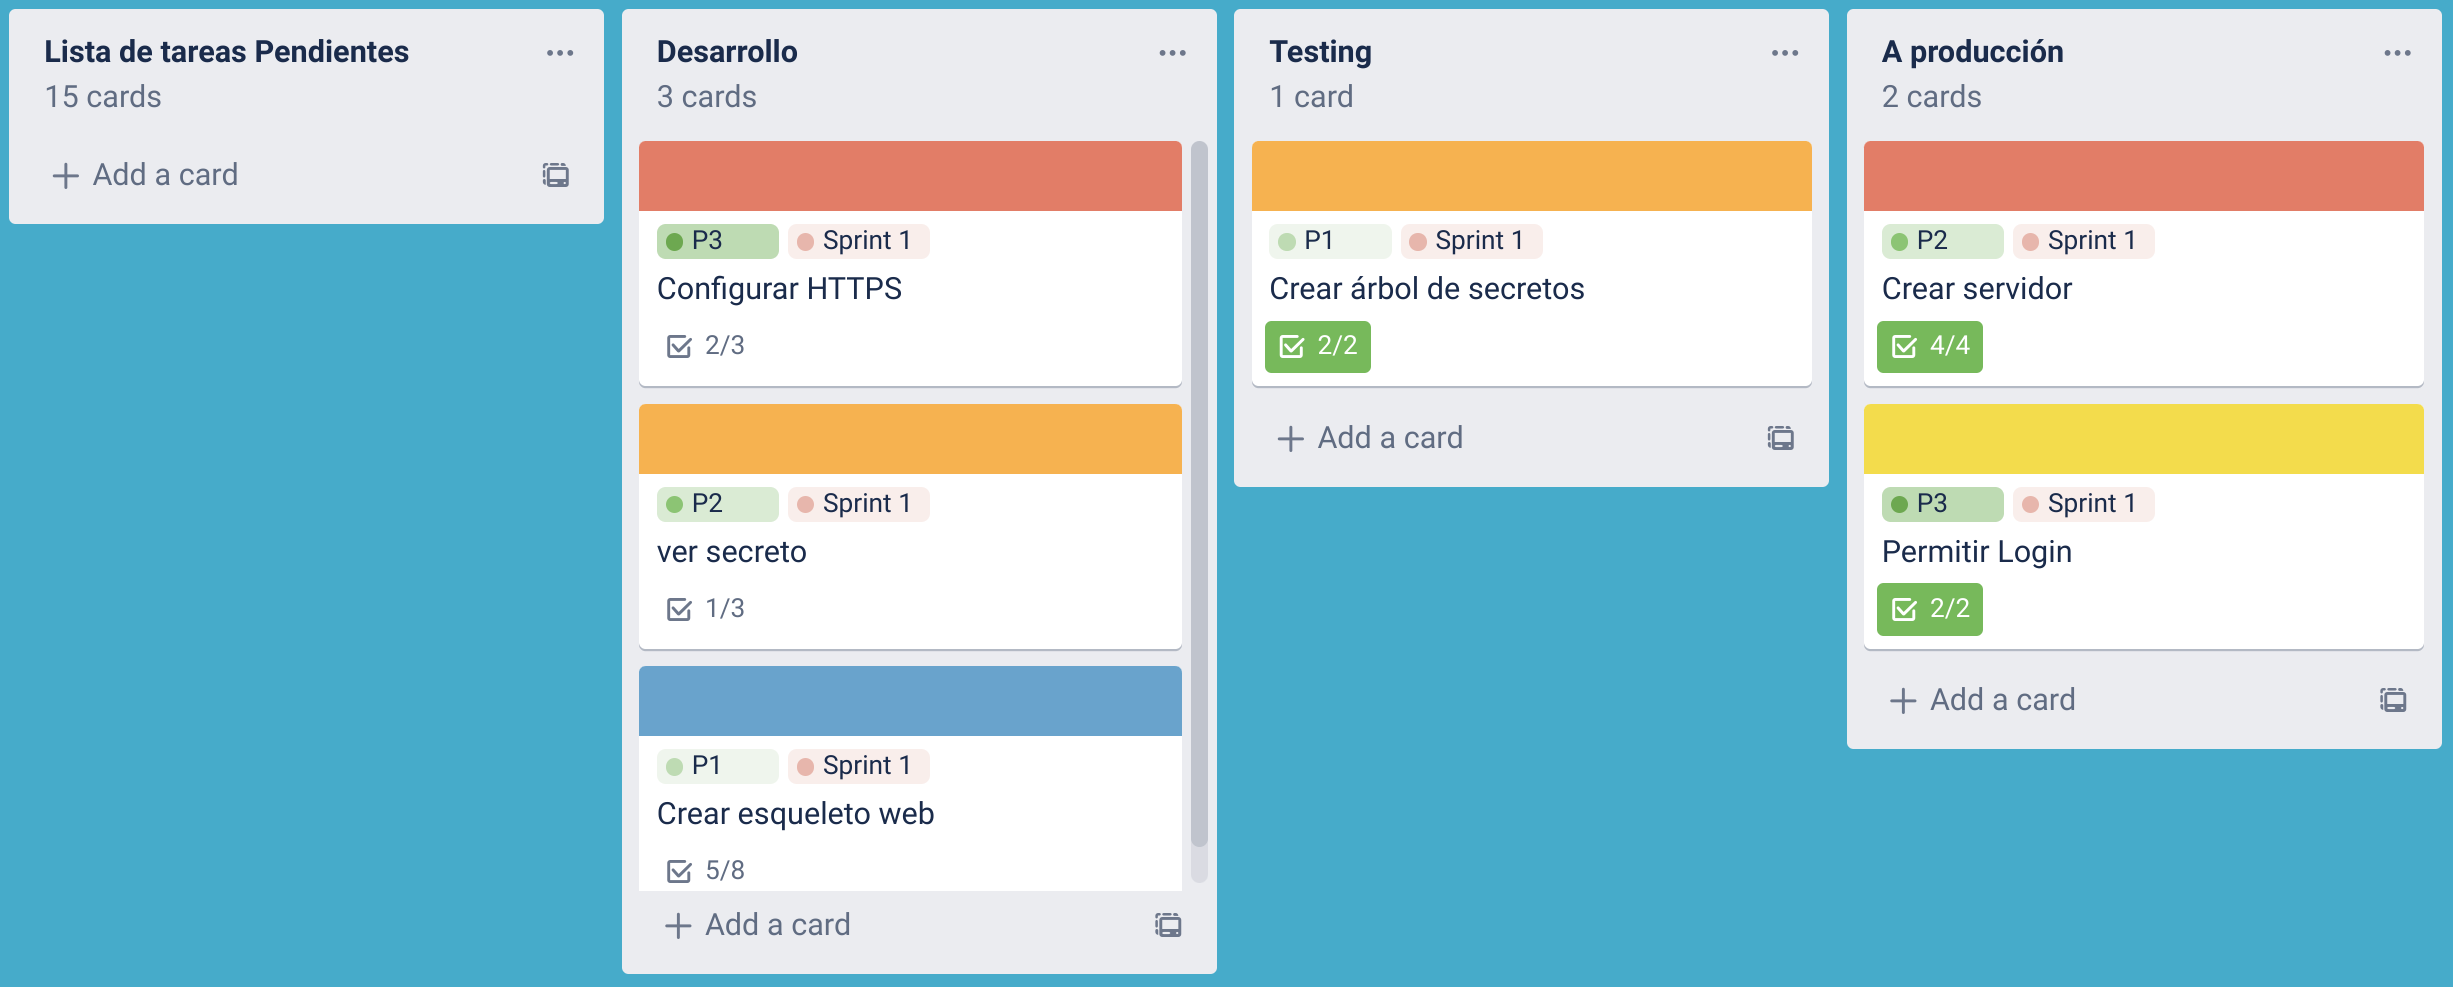
\includegraphics[width=\linewidth]{img/board4.png}
\end{center}
\vspace{-10pt}
Uno de los aspectos principales que podemos ver es que en la columna de tareas pendientes ya no tenemos ninguna del \textit{sprint 1} (sigue habiendo 15 tareas, pero ocultas, que son de los siguientes \textit{sprints}).

Por otro lado, vemos que la tarea “crear esqueleto web” ha vuelto a la columna “desarrollo”, ya que el cliente nos ha otorgado \textit{feedback} y se han añadido nuevos \textit{ítems} (se ha pasado de 5 a 8), y se han identificado como:

\begin{itemize}
    \item El cliente pide: modificar color del background.
    \item El cliente nos da un logotipo nuevo.
    \item El cliente pide cambiar el footer.
\end{itemize}

Estas modificaciones no se habían visto contempladas porque el cliente ha decidido hacer un \textit{rebranding} de su marca y logotipo tras comenzar con el desarrollo de la aplicación, por lo que hay que adaptarse a ello.

Por otro lado, se ha pasado a producción dos tareas (“crear servidor” y “permitir login”), y otra que estaba previamente en desarrollo se ha dado por finalizada comenzando su testeo.


\chapter{Conclusiones}

Tal como se ha podido ver a lo largo del documento, antes de comenzar con el desarrollo de un proyecto hay un trabajo previo que debe realizarse, y que es muy importante como es el de crear las historias de usuario.

Con ellas podremos comenzar a realizar el \textbf{product backlog}, que posteriormente nos permitirá distinguir las distintas tareas y representarlas en los distintos \textit{sprints} que llevaremos a cabo.

Tras esto, herramientas como \href{https://trello.com/}{Trello} nos van a ayudar para que los desarrolladores puedan ver las tareas que deben realizar y cómo se encuentra el estado del \textit{sprint} actual.

\end{document}
